\documentclass[UTF8,fontset=windows,a4paper,11pt]{ctexart}
\usepackage[left=3.1cm,right=3.1cm,top=3.15cm,bottom=2.45cm,headheight=1.18cm,headsep=.42cm]{geometry}
\usepackage{graphicx,booktabs,longtable,array,caption,float,needspace,amssymb,fancyhdr,hyperref}
\usepackage{url}
\hypersetup{unicode=true,hidelinks,breaklinks=true}
\urlstyle{same}
\def\UrlBreaks{\do\/\do\_\do\.\do\-}
\emergencystretch=2em
\setlength{\parindent}{2em}
\setlength{\parskip}{.35em}
\linespread{1.23}
\setlength{\LTpre}{8pt}
\setlength{\LTpost}{10pt}
\captionsetup{font=small,labelfont=bf}
\ctexset{section={format=\Large\bfseries,beforeskip=1.35em,afterskip=.68em},subsection={format=\large\bfseries,beforeskip=1.1em,afterskip=.5em}}
\pagestyle{fancy}
\fancyhf{}
\fancyhead[C]{\small 基于 FPGA 的八角与莽草形态识别系统}
\renewcommand{\headrulewidth}{.4pt}
\fancyfoot[C]{作品设计报告\quad ·\quad 第 \thepage{} 页}
\begin{document}
\begin{center}
{\LARGE\bfseries 基于 FPGA 的八角与莽草形态识别系统\par}
\vspace{.45em}
{\large 作品设计报告\par}
\end{center}


\needspace{5\baselineskip}\section*{摘要}

本作品面向单颗星形果实的视觉形态分析，构建了从 OV5640 摄像头采集、FPGA 图像处理到 HDMI 六画面显示的完整系统。图像计算由可编程逻辑中的 HLS 加速器完成，包括光照补偿、目标分割、内部孔洞填充、径向尖端检测及多帧一致性筛选；处理器端负责设备初始化、帧缓冲管理和任务调度。系统通过按键锁存角数规则对应的分类结果，便于观察处理过程与输出之间的关系。实现报告显示，本版已完成实现与布线，WNS 为 +0.010 ns，WHS 为 +0.008 ns；工程记录板端处理更新速度约为 2.6 次/秒。当前采用少于 10 个角与不少于 10 个角的实验分类规则，尚无覆盖足够多独立实物的准确率证据。本说明书据实记录已实现功能、算法结构、资源使用和验证边界，供竞赛评审及工程复现使用。\par

\noindent\textbf{关键词  FPGA；PYNQ-Z1；光照补偿；形态分析；尖端检测；HLS}

\needspace{5\baselineskip}\section*{第一部分 作品概述}

\needspace{4\baselineskip}\subsection*{1.1 功能与特性}

系统面向固定机位、浅色背景和单颗完整样品。OV5640 采集 640×480 RGB565 图像，板端将输入缩为 160×120 工作图，HLS 加速器完成补光、分割、轮廓和尖端分析；HDMI 同屏显示原图、轮廓、补光、白底分割、候选尖端和稳定尖端。按一次 BTN0 锁存最近结果，再按一次回到 WAIT。输出“八角”“莽草”或无效结果，依据为实验性的角数阈值。\par

表 1 将本系统已实现的功能逐项列出。“\checkmark{}”表示代码中具有对应实现，并纳入最终工程或板端演示链路。勾选不等同于跨实物、跨光照条件下的分类准确率验证。\par

\begin{center}
\begingroup
\fontsize{8.5}{11}\selectfont
\setlength{\tabcolsep}{3pt}
\renewcommand{\arraystretch}{1.22}
\begin{longtable}{@{}p{2.836cm}p{6.617cm}p{0.945cm}p{3.402cm}@{}}
\caption{本系统功能核对}\\
\toprule
\textbf{功能项} & \textbf{本版实现内容} & \textbf{完成} & \textbf{核验依据} \\
\midrule
\endfirsthead
\toprule
\textbf{功能项} & \textbf{本版实现内容} & \textbf{完成} & \textbf{核验依据} \\
\midrule
\endhead
\bottomrule
\endfoot
摄像头采集 & OV5640 DVP 输入，640×480 RGB565 & \checkmark{} & 源码、实机画面 \\
图像缩小 & 4×4 稀疏采样为 160×120 工作图 & \checkmark{} & HLS 源码 \\
光照补偿 & 对工作图进行亮度补偿并展示结果 & \checkmark{} & HLS 源码、六画面 \\
目标分割 & 亮度与色度两条分割路径生成目标掩膜 & \checkmark{} & HLS 源码、六画面 \\
掩膜修复 & 对前景内部孔洞填充及噪点处理 & \checkmark{} & HLS 源码 \\
轮廓提取 & 显示目标边缘并生成径向轮廓数据 & \checkmark{} & HLS 源码、六画面 \\
候选尖端检测 & 根据径向峰检测候选尖端位置 & \checkmark{} & HLS 源码、六画面 \\
多帧稳定筛选 & 在最多九帧历史中按尖端位置一致性筛选 & \checkmark{} & HLS 源码 \\
实验性分类 & 有效目标下按角数阈值输出八角或莽草 & \checkmark{} & RTL 源码、板端画面 \\
无效目标处理 & 无效样品输出未识别状态 & \checkmark{} & RTL 源码 \\
六画面 HDMI & 同时显示原图和五类处理结果 & \checkmark{} & 实机视频截帧 \\
按键结果锁存 & BTN0 锁存结果，再次按下返回 WAIT & \checkmark{} & RTL 源码、仿真 \\
板端管理 & PYNQ Linux 配置摄像头、VDMA 和缓冲区 & \checkmark{} & 板端 Python \\
\end{longtable}
\endgroup
\end{center}

\needspace{4\baselineskip}\subsection*{1.2 应用领域与选题背景}

八角与外形相近的星形果实容易受到阴影、姿态和缺损影响。已有视觉思路包括直接训练分类网络，以及先分割目标、再依据轮廓和凸起位置判断。本团队前期试过 CNN 方案，但同一实物的多张照片不足以证明对新实物的泛化能力。本系统聚焦可解释的板端形态分析：把每一步中间图显示出来，便于发现误分割和漏检。当前适合教学演示、算法验证及受控场景的形态筛查，不用于药材安全判定。\par

\needspace{4\baselineskip}\subsection*{1.3 主要技术特点}

本版把补光、双分支目标分割、孔洞填充、径向峰检测和最多九帧的位置一致性筛选实现在 PL 侧 HLS 加速器中。PS 端 Python 只管理摄像头配置、DDR 帧缓冲、VDMA 与加速器启动。分类比较和按键锁存在 RTL 中完成。六画面共用一次处理结果，便于把输入、掩膜和尖端逐步对照。所有结论以随包代码、实现报告和既有实机画面为依据。\par

\needspace{4\baselineskip}\subsection*{1.4 主要性能指标}

\begin{center}
\begingroup
\fontsize{8.5}{11}\selectfont
\setlength{\tabcolsep}{3pt}
\renewcommand{\arraystretch}{1.22}
\begin{longtable}{@{}p{3.024cm}p{4.158cm}p{6.617cm}@{}}
\caption{主要性能指标与证据边界}\\
\toprule
\textbf{指标} & \textbf{当前结果} & \textbf{证据或边界} \\
\midrule
\endfirsthead
\toprule
\textbf{指标} & \textbf{当前结果} & \textbf{证据或边界} \\
\midrule
\endhead
\bottomrule
\endfoot
输入与输出 & 640×480 RGB565；720p HDMI & 工程源码及约束 \\
工作图 & 160×120 & HLS 源码；4×4 稀疏采样 \\
处理更新 & 约 2.6 次/秒 & 工程记录，非本次重新实测 \\
时序 & WNS +0.010 ns；WHS +0.008 ns & 最终实现报告 \\
分类准确率 & 未给出 & 缺少独立实物真值与混淆矩阵 \\
\end{longtable}
\endgroup
\end{center}

\needspace{4\baselineskip}\subsection*{1.5 主要创新点}

一是将光照补偿、分割和数角过程同时可视化，使误判位置可追踪。二是用亮度与色度两条分割路径适应不同背景亮度。三是用归一化尖端位置而非预设角度或固定角数做最多九帧的历史一致性筛选。这些是本作品的设计特点，尚未证明相对已有方法的领先性能。\par

\needspace{4\baselineskip}\subsection*{1.6 设计流程}

先完成摄像头、VDMA 与 HDMI 链路，再用实物图像验证补光和分割；随后在 PC 端观察尖端漏检，确定径向峰与多帧筛选规则；将算法移入 HLS，分类和锁存写成 RTL；最后执行 Vivado 综合、布局布线和板端六画面演示。\par

\needspace{5\baselineskip}\section*{第二部分 系统组成及功能说明}

\needspace{4\baselineskip}\subsection*{2.1 整体介绍与功能框图}

Zynq 的处理器系统 PS 运行 PYNQ Linux，可编程逻辑 PL 执行图像运算和视频接口功能。该设计采用 DDR 帧缓冲架构：摄像头持续采集，软件选择已完成帧并复制到快照缓冲，随后启动 HLS；HLS 完成整帧拼接后，软件将结果提交给显示 VDMA。\par

\begin{figure}[H]
\centering
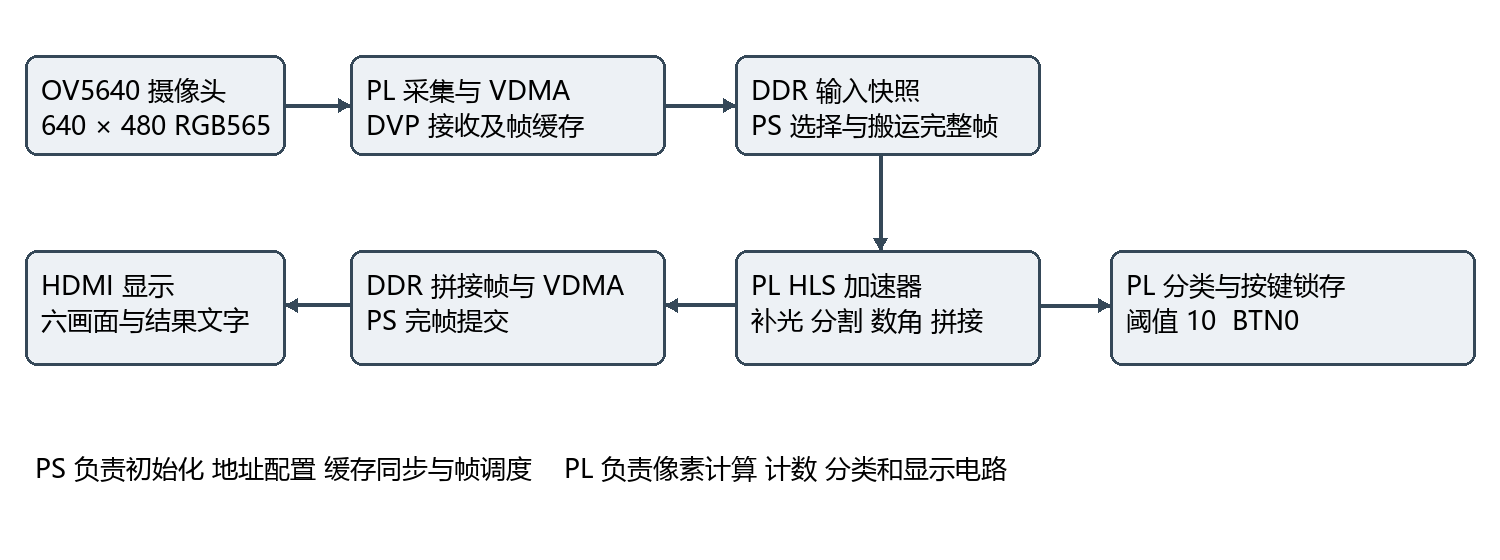
\includegraphics[width=0.94\linewidth,keepaspectratio]{figures/architecture.png}
\caption*{图 1  帧式软硬件协同数据流}
\end{figure}

摄像头视频和显示视频由 PL 的 VDMA 连续搬运。每一次算法更新，PS 从采集环帧复制一幅快照至独立输入缓冲，设置 HLS 地址，等候加速器结束，再把拼接图复制到显示帧并按帧边界提交。四个 HLS m\_axi 端口最终汇入共享的 PS HP0 DDR 通道，因此接口数量并不等于四条独立内存通道。\par

软件中存在 NumPy 帧复制及缓存 flush / invalidate 操作，瓶颈既可能在 HLS 内核，也可能在 CPU 搬运与 DDR 竞争。HDMI 的名义 60 Hz 时序只是输出刷新速率，不能代表识别更新速率。\par

\needspace{4\baselineskip}\subsection*{2.2 硬件系统}

硬件由 PYNQ-Z1、OV5640 DVP 摄像头、固定样品台和 HDMI 显示器组成。摄像头经 SCCB/I²C 初始化，DVP 数据在 PL 侧接收并跨时钟缓存；显示电路以固定 720p 时序读取已完成的拼接帧。样品台使用简易固定结构，没有自制 PCB 或舵机分拣机构，因此不提供不存在的 SCH、PCB 或机械加工图。\par

\begin{center}
\begingroup
\fontsize{8.5}{11}\selectfont
\setlength{\tabcolsep}{3pt}
\renewcommand{\arraystretch}{1.22}
\begin{longtable}{@{}p{3.403cm}p{4.915cm}p{5.482cm}@{}}
\caption{硬件与软件模块职责}\\
\toprule
\textbf{模块} & \textbf{职责} & \textbf{实现依据} \\
\midrule
\endfirsthead
\toprule
\textbf{模块} & \textbf{职责} & \textbf{实现依据} \\
\midrule
\endhead
\bottomrule
\endfoot
DVP 接收与跨时钟缓存 & 接收 RGB565 并向视频总线输出 & dvp\_rgb565\_rx.v 及 Vivado BD \\
HLS 加速器 & 补光、分割、尖端检测、拼接 & sixpanel\_accel.cpp \\
分类器与交互 & 按计数分类，按键消抖与结果锁存 & vision\_tip\_count\_classifier.v 等 \\
显示链路 & 读取拼接图、720p 时序与文字叠加 & hdmi\_vga\_axis\_raster.v 等 \\
PS 运行程序 & 配置摄像头、分配缓存、启动与监控 & board\_fpga\_sixpanel.py \\
\end{longtable}
\endgroup
\end{center}

图 2、图 3 是实物近景，分别展示开发板与摄像头模组的连接状态。两图仅用于说明硬件组成与接线方式，不作为图像算法性能或分类正确率的证据。\par

\begin{figure}[H]
\centering
\begin{minipage}[t]{0.47\linewidth}\centering
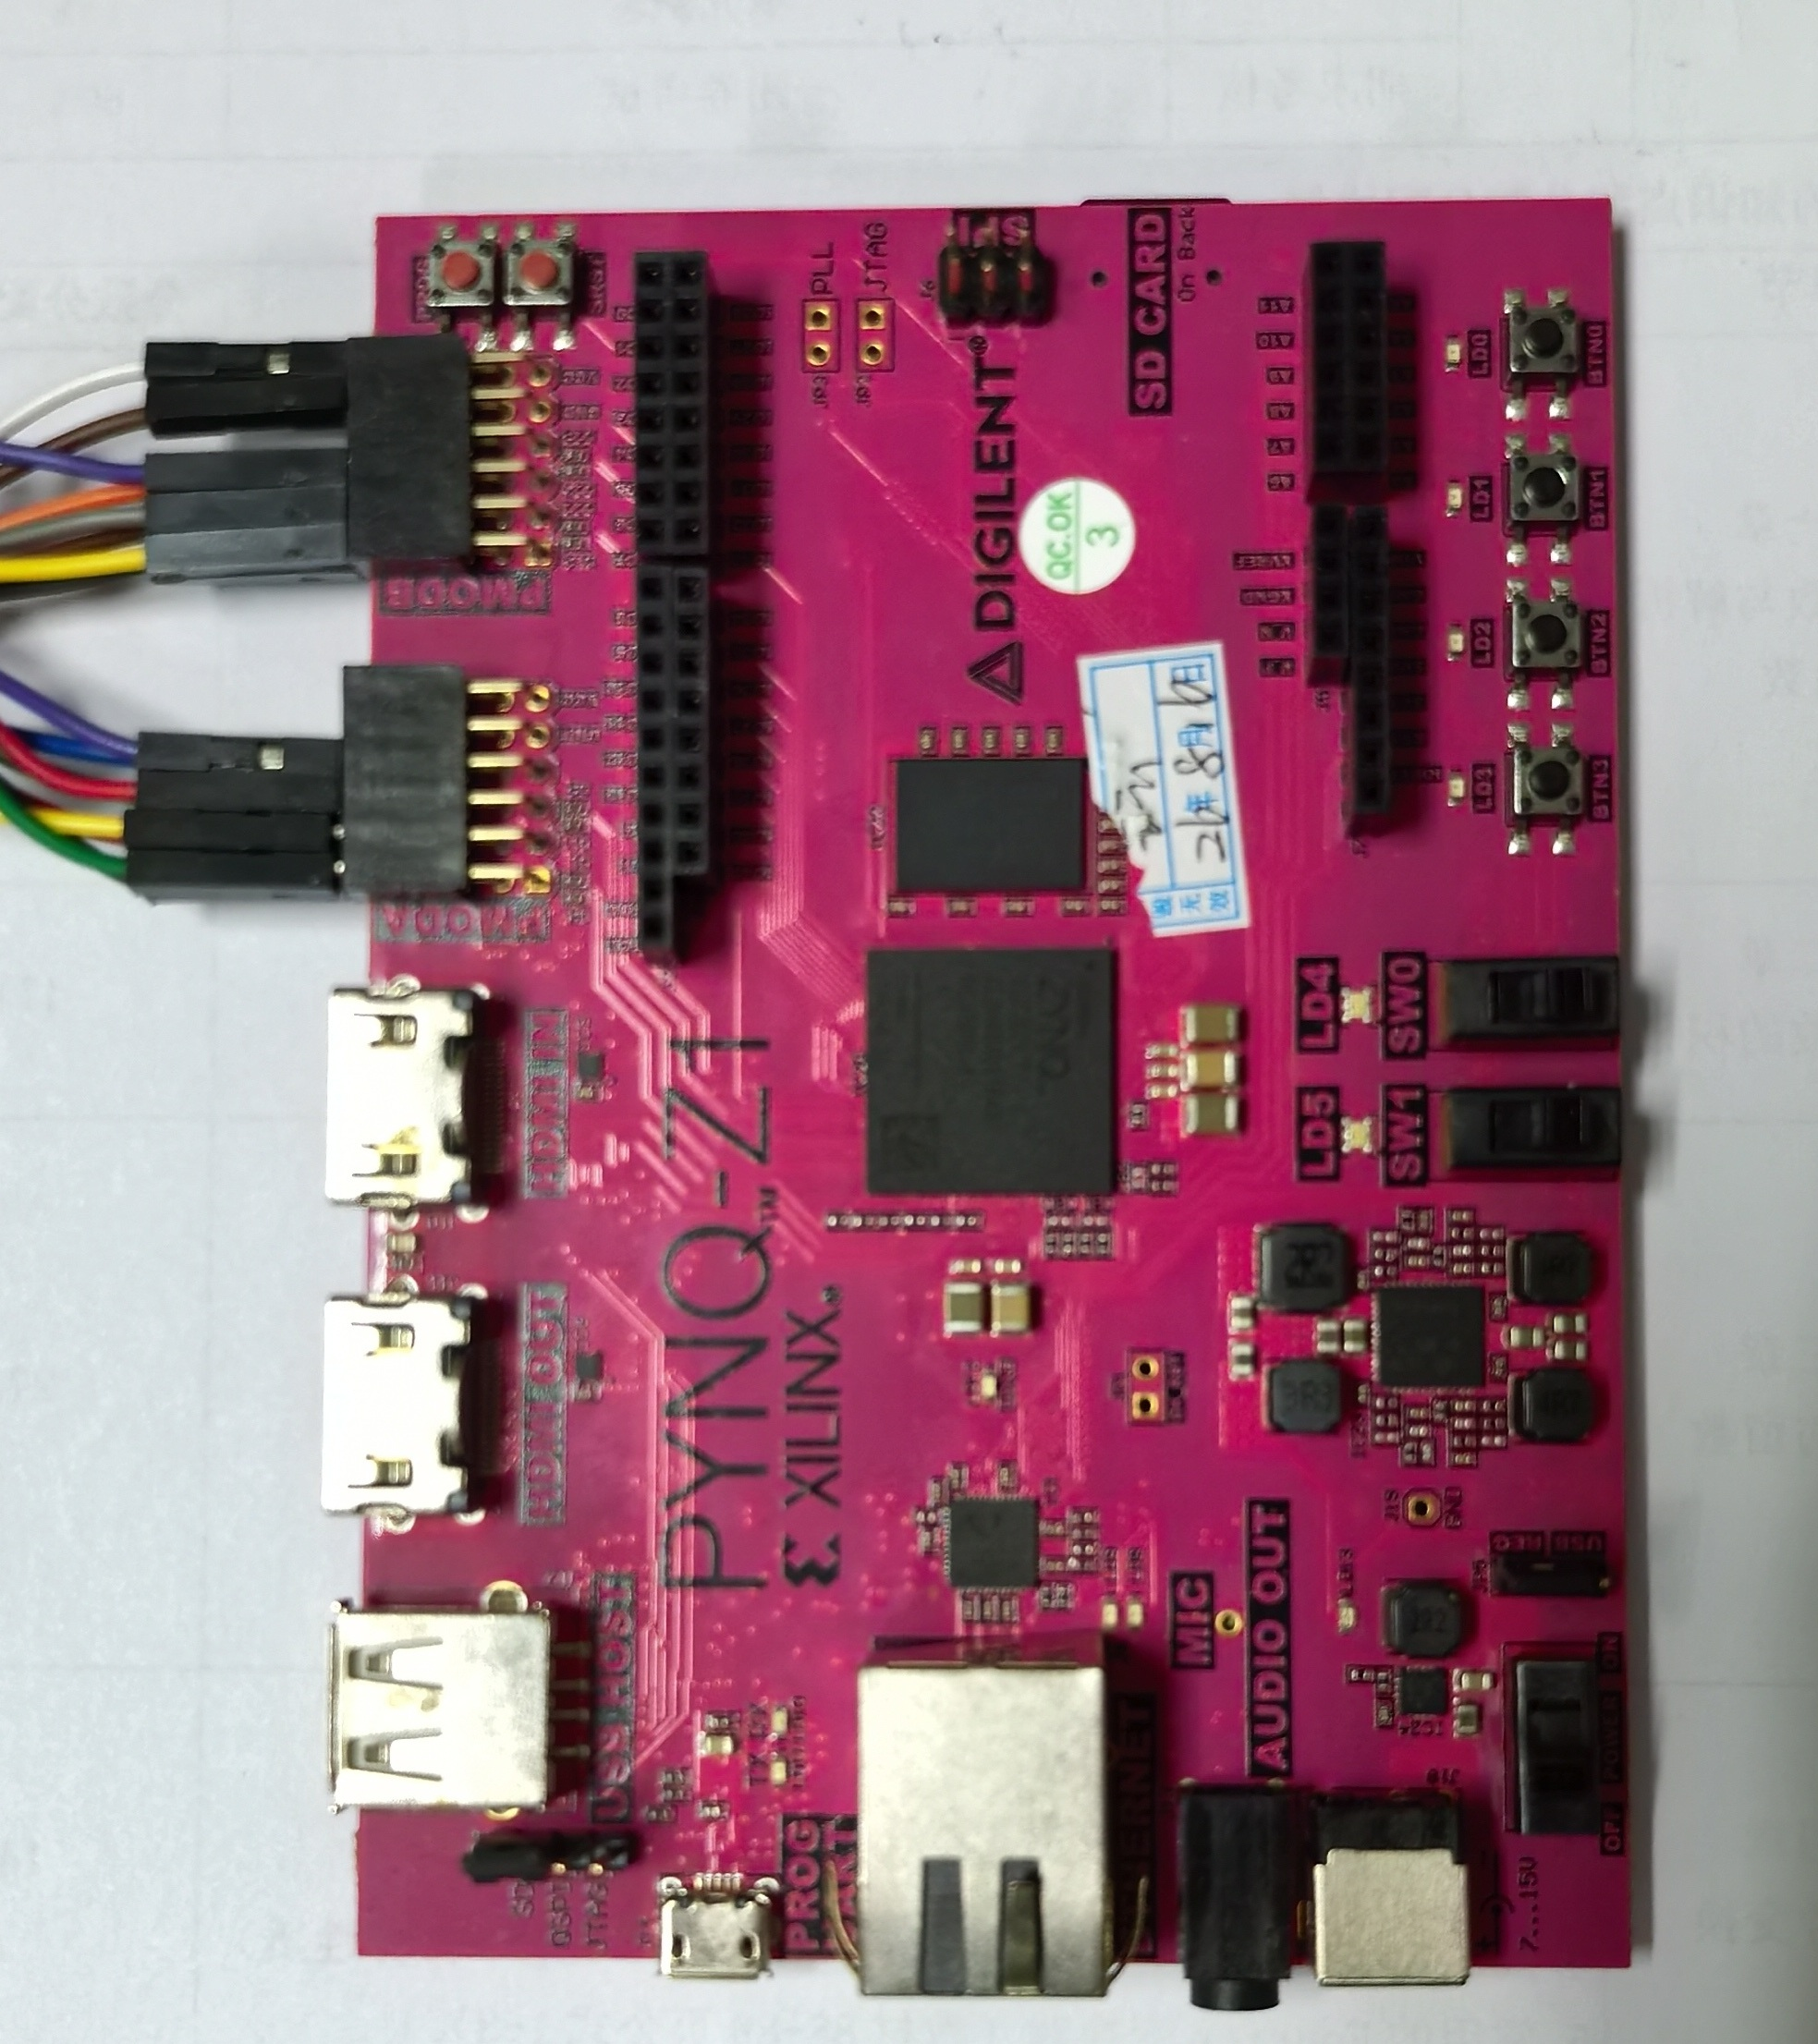
\includegraphics[width=\linewidth,height=5.4cm,keepaspectratio]{figures/board_closeup.jpg}
\caption*{图 2  PYNQ-Z1 与摄像头线束连接近景}
\end{minipage}\hfill
\begin{minipage}[t]{0.47\linewidth}\centering
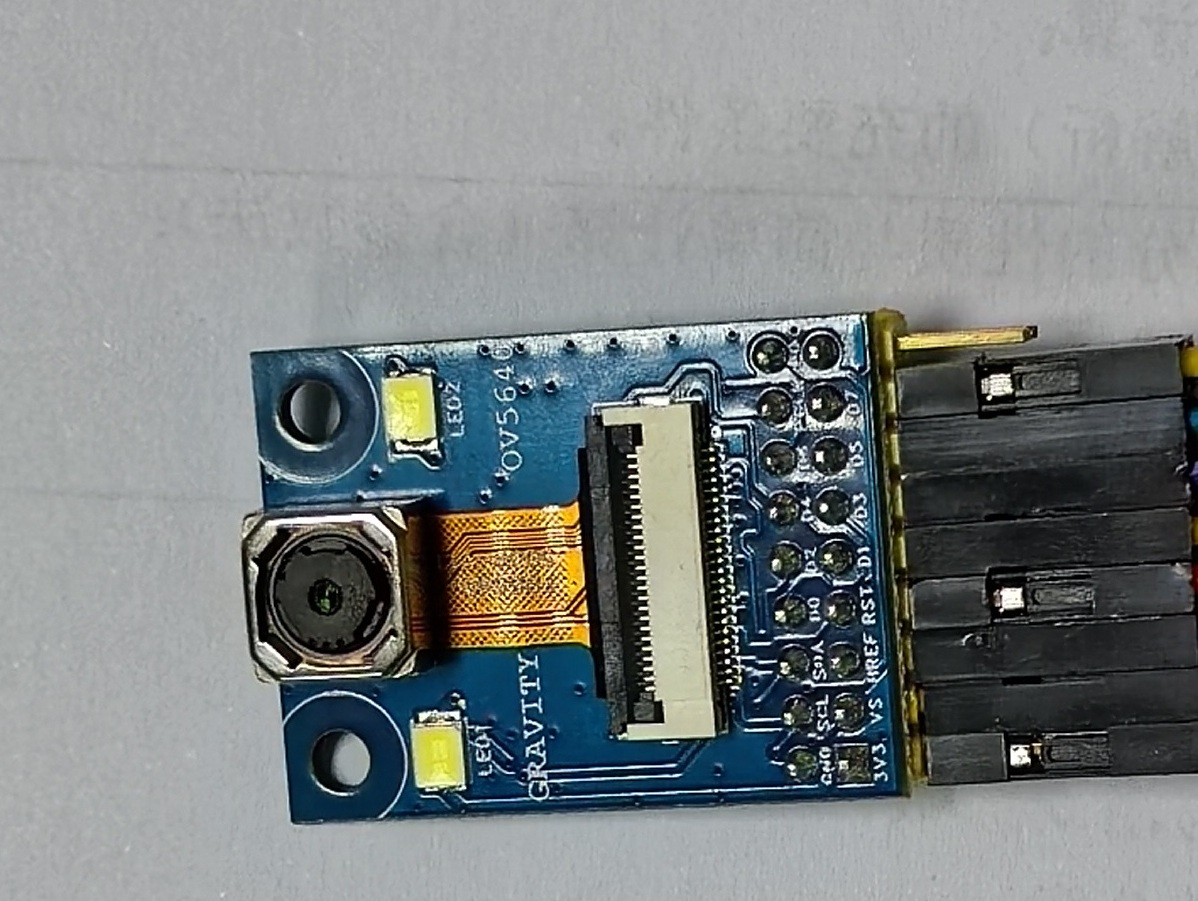
\includegraphics[width=\linewidth,height=5.4cm,keepaspectratio]{figures/camera_closeup.jpg}
\caption*{图 3  OV5640 摄像头模组与线束近景}
\end{minipage}
\end{figure}

\needspace{4\baselineskip}\subsection*{2.2.1 关键接口与信号}

\begin{center}
\begingroup
\fontsize{8.5}{11}\selectfont
\setlength{\tabcolsep}{3pt}
\renewcommand{\arraystretch}{1.22}
\begin{longtable}{@{}p{2.930cm}p{5.388cm}p{5.483cm}@{}}
\caption{关键接口与信号}\\
\toprule
\textbf{接口} & \textbf{输入与输出} & \textbf{功能} \\
\midrule
\endfirsthead
\toprule
\textbf{接口} & \textbf{输入与输出} & \textbf{功能} \\
\midrule
\endhead
\bottomrule
\endfoot
OV5640 DVP & D0–D7、PCLK、HREF、VSYNC $\rightarrow$ PL & 接收 RGB565 像素和行帧时序 \\
摄像头控制 & AXI IIC 的 SCL/SDA；RST GPIO & 配置寄存器和复位摄像头 \\
HLS DDR 接口 & 4 组 m\_axi；共享 PS HP0 通道 & 读输入快照，写六画面、历史及工作区 \\
HLS 控制接口 & AXI-Lite 地址与 ap\_start/ap\_done & PS 启动和等待整帧处理 \\
结果直连 & stable\_tip\_count、detector\_valid、frame\_done & 驱动角数分类与按键锁存 RTL \\
HDMI 与按键 & 拼接帧 $\rightarrow$ HDMI；BTN0 $\rightarrow$ 同步消抖 & 六画面、结果文字及人工锁存 \\
\end{longtable}
\endgroup
\end{center}

\needspace{4\baselineskip}\subsection*{2.2.2 光照补偿、分割与尖端算法}

640 × 480 输入按每个 4 × 4 区域中的四个指定位置取样并求均值，形成 160 × 120 工作图像。它减少后续存储和运算，但并非对全部 16 个像素做面积平均，也不采用早期方案中的 244 × 244 CNN 输入。\par

补光首先提取 HSV 的 V 分量，再以 49 抽头的一维高斯近似核分别进行水平与垂直滤波，估计缓慢变化的照度分布 L。系数使用 Q12 定点表示。取照度直方图中位数作为参考亮度 R，再计算每个位置的增益。\par

算法表达为 g = clip(R / max(L, 24), 154/256, 563/256)，$V^{\prime}$ = clip(V × g, 0, 255)。R 是当前帧照度的中位数，L 是该像素周围的平滑照度；Q8 增益的实际范围约为 0.60～2.20。低照度分母钳位抑制噪声放大，增益上下限防止过亮和过暗区域过度修正。此处理减弱缓变阴影，不能恢复被遮挡或饱和丢失的纹理。\par

补光结果进入容量为 5 帧的历史缓存，各 RGB 通道分别计算历史中位数，抑制静止物体画面的瞬时波动。稳定图像优先进入暗目标分支：用四周 10 像素边带的灰度中位数估计背景亮度，阈值取该亮度的 62\%，并保留最大连通域。\par

暗目标分支要求背景亮度至少为 48，目标面积至少 100 像素且小于工作图像的三分之一，外接框宽高差均至少为 12 像素，同时满足内部边界约束。条件不满足时，切换到色度分支；分支切换会清空尖端历史，减少不同掩膜混用。\par

色度分支将 RGB 各通道除以该像素的最大通道值再缩放到 255，以降低整体亮度的影响。之后执行 5 × 5 双边滤波近似，使用空间权重和查表的颜色距离权重。每行两端各取 20 个像素估计背景色相，以 11 行中值平滑基线；圆周色相差不小于 12 且饱和度不小于 40 的像素进入候选前景。\par

候选掩膜经 3 × 3 开运算、5 × 5 闭运算及最大连通域筛选。两条分支最后均执行内部孔洞填充，把与图像外部背景不连通的孔洞合并到前景。轮廓显示直接从该掩膜提取边界，便于发现投影粘连或真实尖端被抹去等问题。\par

对最终二值掩膜求面积质心，坐标以 Q8 定点表示。将掩膜与其 3 × 3 腐蚀结果相减获得边界；依据边界点相对质心的方向，把它们映射至 360 个角度桶，每桶保存最远边界点。角度由反正切查表和象限判断得到，距离使用 max(|dx|, |dy|) + 106 × min(|dx|, |dy|) / 256 的近似式，避免直接求平方根。\par

若不足 180 个方向有有效边界数据，本帧不输出尖端。其余缺失角度通过相邻有效方向插值填补；随后采用 13 抽头周期平滑核抑制轮廓锯齿，使圆周起点与终点连续。\par

算法在平滑后的径向曲线上寻找局部峰，左右各检查 9 个角度桶，并计算峰顶相对两侧谷底的突出程度。突出度阈值随半径分布变化，最低阈值为 90 个 Q8 单位。候选峰按半径和突出度选优，保留峰的角度间隔至少为 18°，输出数组容量为 32 个。该方法依赖真实尖端在质心径向曲线上形成可分离峰。\par

候选尖端以质心和尺度归一化后写入容量为 9 帧的环形历史。当前候选点与历史点的归一化距离平方不大于 46² 时计为一次匹配；匹配次数须达到 ceil(历史帧数 × 55\%)，且至少为 2 次。输出由此得到的稳定尖端数，检测有效条件为存在目标外接框且稳定尖端数大于 0。\par

时间匹配依据归一化后的尖端坐标，不是对九次角数做简单多数投票，也没有预先指定角数或方向。它可以抑制随机跳动，但稳定的错误轮廓同样可能被保留。算法没有显式的实物身份跟踪；更换样品、旋转或大幅移动时，须等待历史重新积累，再触发锁存。\par

该分类器没有训练权重，也没有概率置信度输出。早期 CNN 的准确率、置信度差阈值和训练集测试结果不适用于本版，不能直接移入本报告。\par

\needspace{4\baselineskip}\subsection*{2.3 软件系统与函数接口}

板端运行 PYNQ Linux 3.1.1。\path{board_fpga_sixpanel.py} 加载与 \path{.bit} 同名的 \path{.hwh}，配置摄像头、VDMA 和 HLS 寄存器，分配输入快照、拼接暂存、历史和工作缓冲。\path{ov5640_vga_720p_hdmi.py} 负责摄像头初始化与状态读取。PC 端的 \path{board_vision_algorithms.py} 是算法参考代码，不是最终板端逐像素实时执行路径。\par

\begin{center}
\begingroup
\fontsize{8.5}{11}\selectfont
\setlength{\tabcolsep}{3pt}
\renewcommand{\arraystretch}{1.22}
\begin{longtable}{@{}p{3.970cm}p{4.915cm}p{4.915cm}@{}}
\caption{板端缓冲区分配}\\
\toprule
\textbf{缓冲区} & \textbf{软件分配} & \textbf{字节数} \\
\midrule
\endfirsthead
\toprule
\textbf{缓冲区} & \textbf{软件分配} & \textbf{字节数} \\
\midrule
\endhead
\bottomrule
\endfoot
输入快照 & 307200 × uint16 & 614400 \\
拼接暂存 & 819200 × uint16 & 1638400 \\
补光历史 & 96000 × uint32 & 384000 \\
工作区 & 900000 × uint32 & 3600000 \\
上述合计 & 不含 VDMA 帧环与系统内存 & 6236800 \\
\end{longtable}
\endgroup
\end{center}

\begin{center}
\begingroup
\fontsize{8}{10}\selectfont
\setlength{\tabcolsep}{3pt}
\renewcommand{\arraystretch}{1.05}
\begin{longtable}{@{}p{3.686cm}p{4.727cm}p{5.387cm}@{}}
\caption{软件函数与模块接口}\\
\toprule
\textbf{函数或模块} & \textbf{关键输入} & \textbf{关键输出或作用} \\
\midrule
\endfirsthead
\toprule
\textbf{函数或模块} & \textbf{关键输入} & \textbf{关键输出或作用} \\
\midrule
\endhead
\bottomrule
\endfoot
\path{main()} & Overlay、摄像头及 DDR 地址 & 启动采集和显示，逐帧调度 HLS \\
\path{_write_address()} & MMIO、寄存器偏移、物理地址 & 向 AXI-Lite 写入 64 位缓冲地址 \\
\path{camera_reset_and_check()} & GPIO、AXI IIC & 复位并检查 OV5640 \\
\path{sixpanel_accel()} & RGB565 快照、历史和工作区 & 拼接图、稳定角数、有效与完成信号 \\
\end{longtable}
\endgroup
\end{center}

为保证帧完整性与交互一致性，HLS 写入独立的拼接暂存区，完成后才由软件复制到显示帧并在帧边界提交，避免显示器扫描未完成的中间画面。BTN0 输入经两级同步和默认 20 ms 消抖。第一次按下锁存最近完成的类别，第二次回到 WAIT；六画面仍连续更新，右下角 TIPS 可能与锁存时的类别来自不同更新时刻。演示时应按“等待稳定$\rightarrow$按键锁存$\rightarrow$查看画面”顺序操作。\par

\needspace{4\baselineskip}\subsection*{2.4 资源与性能优化}

大幅 RGB 图像、六幅显示图块、连通域标签及队列放入 DDR 工作区；高频访问的灰度、掩膜及部分处理缓存保留在片上。数组视图传入辅助函数，避免把所有完整工作帧推断为 BRAM。小位宽掩膜采用 ap\_uint<1> 表示，降低逻辑存储需求。RGB 与 HSV 转换中的部分小范围除法使用 Q24 倒数查表、乘法和余数修正，替代通用除法器。乘法中间结果使用 64 位防止移位前溢出。角度使用查表，径向距离使用加法和定系数近似。2 倍显示放大的双线性权重利用四分之一与四分之三的关系改成移位加法。320 × 240 图块铺满最终六画面时，为减少 DDR 读流量，末级缩放实际采用单点采样；相关函数虽名为 bilinear\_panel，行为应以函数体为准。源码中的 PIPELINE II=1 是局部循环优化目标，不能由此推导整条处理链每周期一像素。\par

下表按“原规划或可比较方法—最终实现”记录优化过程。现有工程资料没有同输入、同时钟、同工具设置的优化前完整实现报告，因而不能把当前资源占用与某个历史工程相减并声称节省比例；表中的前后性能与资源比较以可核验范围为限。\par

\begin{center}
\begingroup
\fontsize{8.5}{11}\selectfont
\setlength{\tabcolsep}{3pt}
\renewcommand{\arraystretch}{1.22}
\begin{longtable}{@{}p{2.269cm}p{3.591cm}p{3.970cm}p{3.970cm}@{}}
\caption{资源与性能优化对照}\\
\toprule
\textbf{优化点} & \textbf{原规划或候选方案} & \textbf{最终实现} & \textbf{可量化结论} \\
\midrule
\endfirsthead
\toprule
\textbf{优化点} & \textbf{原规划或候选方案} & \textbf{最终实现} & \textbf{可量化结论} \\
\midrule
\endhead
\bottomrule
\endfoot
工作分辨率 & 按 640×480 全帧处理 & 4×4 稀疏采样为 160×120 & 主算法工作像素数变为 1/16；不是整机加速倍数 \\
大帧存储 & 大数组集中留在片上 & 显示图块与连通域工作区转入 DDR & 最终 BRAM 81/140；缺同条件前版报告 \\
可变除法 & 通用除法器 & Q24 倒数查表及余数修正 & 最终 LUT 35954/53200；单项节省量未测 \\
几何计算 & 直接反正切与平方根 & 角度查表、径向距离近似 & 需与软件基准测误差；无单项资源对照 \\
整机处理 & 早期目标为实时全帧率 & 帧式 HLS 与 DDR 交互 & 约 2.6 次/秒；无同条件前版速度 \\
\end{longtable}
\endgroup
\end{center}

\clearpage

\needspace{5\baselineskip}\section*{第三部分 完成情况及性能参数}

\needspace{4\baselineskip}\subsection*{3.1 实机整体与工程成果}

\begin{figure}[H]
\centering
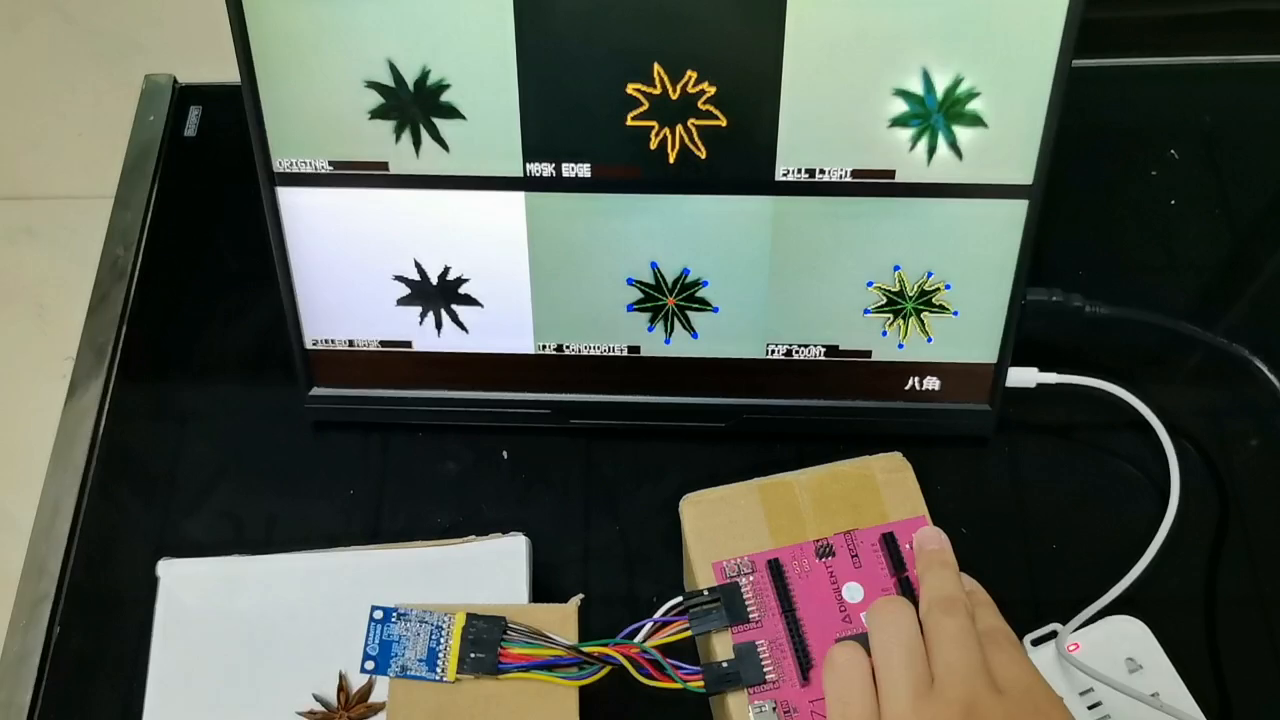
\includegraphics[width=0.83\linewidth,keepaspectratio]{figures/hardware_overview.png}
\caption*{图 4  实机布置与六画面输出  实拍视频截帧}
\end{figure}

图 4 来自实机演示视频截帧，可见显示器、PYNQ-Z1、摄像头连接与单颗样品台。此图是现场工作状态，不代表定型外壳或机械结构验收。\par

工程文件包括可加载的同名 \path{.bit/.hwh}、HLS 图像处理源码、采集与 HDMI RTL、约束、板端启动程序以及最终实现报告。板端和显示程序没有舵机自动分拣，也不运行 CNN 推理。\par

\begin{figure}[H]
\centering
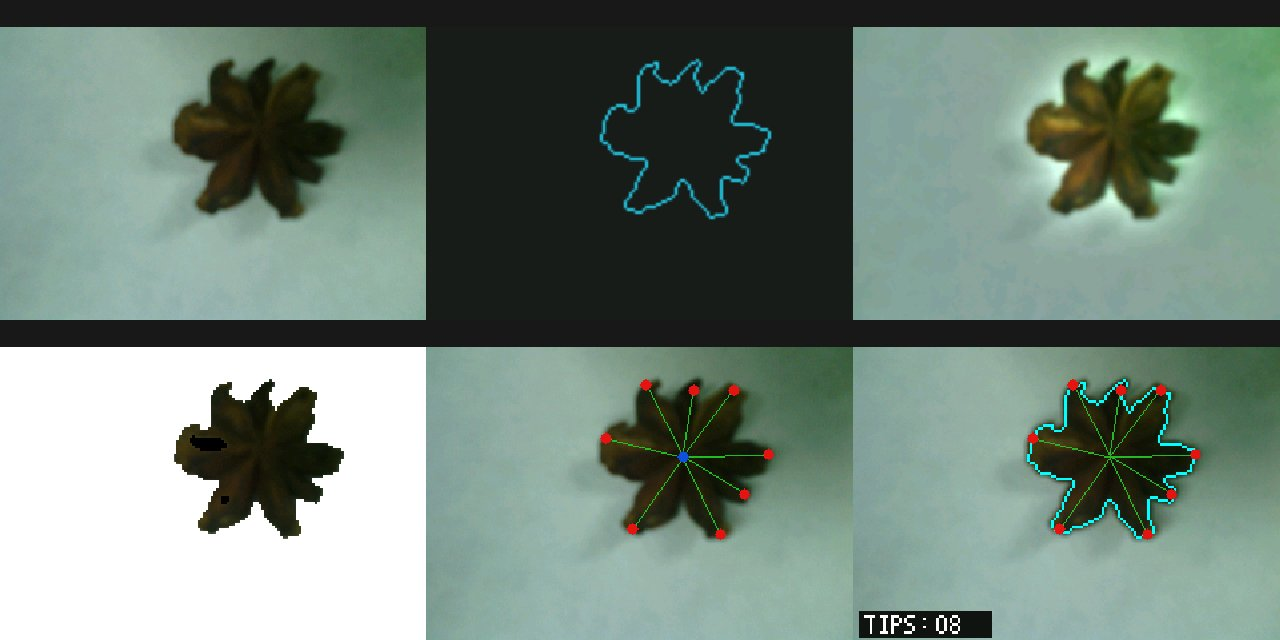
\includegraphics[width=0.94\linewidth,keepaspectratio]{figures/six_panel.jpg}
\caption*{图 5  既有帧缓冲截图  不含 HDMI 后级按键文字叠加}
\end{figure}

截图中可见 TIPS 08，但单张截图不能证明全部样品的计数准确性。包内说明明确该图来自之前一次帧缓冲采集，且不包含 HDMI 后级叠加的按键分类文字，不能把它用作最终中文标签与按键功能的完整验收证据。\par

\needspace{4\baselineskip}\subsection*{3.2 资源、时序与功能验证}

\begin{center}
\begingroup
\fontsize{8.5}{11}\selectfont
\setlength{\tabcolsep}{3pt}
\renewcommand{\arraystretch}{1.22}
\begin{longtable}{@{}p{4.253cm}p{3.024cm}p{3.024cm}p{3.498cm}@{}}
\caption{最终实现资源占用}\\
\toprule
\textbf{资源} & \textbf{使用量} & \textbf{器件总量} & \textbf{占用率} \\
\midrule
\endfirsthead
\toprule
\textbf{资源} & \textbf{使用量} & \textbf{器件总量} & \textbf{占用率} \\
\midrule
\endhead
\bottomrule
\endfoot
Slice LUTs & 35954 & 53200 & 67.58\% \\
Slice Registers & 44973 & 106400 & 42.27\% \\
Block RAM Tile & 81 & 140 & 57.86\% \\
DSPs & 96 & 220 & 43.64\% \\
Slice & 13050 & 13300 & 98.12\% \\
\end{longtable}
\endgroup
\end{center}

\begin{center}
\begingroup
\fontsize{8.5}{11}\selectfont
\setlength{\tabcolsep}{3pt}
\renewcommand{\arraystretch}{1.22}
\begin{longtable}{@{}p{3.024cm}p{4.065cm}p{6.711cm}@{}}
\caption{时序与功能验证结果}\\
\toprule
\textbf{指标} & \textbf{结果} & \textbf{依据及含义} \\
\midrule
\endfirsthead
\toprule
\textbf{指标} & \textbf{结果} & \textbf{依据及含义} \\
\midrule
\endhead
\bottomrule
\endfoot
WNS / TNS & +0.010 ns / 0 & 建立时间满足当前约束，裕量很小 \\
WHS / THS & +0.008 ns / 0 & 保持时间满足当前约束，裕量很小 \\
主要时钟 & 100 MHz / 74.25 MHz / 371.25 MHz & 处理器导出逻辑时钟 / 像素 / 串行化时钟 \\
DRC 与布线 & 报告未列 Error；已有多项 Warning & DRC 警告含检查条目数量封顶提示，须逐项留档 \\
处理更新速度 & 约 2.6 帧/秒 & 工程记录；非本次计时实测 \\
分类准确率 & 尚无可报告数值 & 缺少独立实物真值及混淆矩阵 \\
\end{longtable}
\endgroup
\end{center}

Slice 表示被占用的物理切片，不能与 LUT 百分比混为一谈。本版 Slice 使用接近器件上限，LUT 与 BRAM 均高于 50\%，因此没有实现“各资源均低于 50\%”这一早期目标。已有优化说明了实现方法，但缺少统一条件的优化前基线报告，不能给出可靠的资源节省百分比或加速倍数。\par

板端脚本的 update\_fps 根据循环完成帧数与时间计算。名为 last\_kernel\_ms 的日志计时还包含 HLS 完成后的输出搬运与提交过程，不能直接当作纯 HLS 核执行时间。约 2.6 帧/秒对应约 385 ms 的平均更新周期，只是倒数换算，不是实测端到端识别延迟。\par

包内有除法、孔洞、径向检测的 C++ 检查源码及按键仿真 testbench。按键 testbench 覆盖 9$\rightarrow$八角、锁存后输入变为 12 而类别保持、再次按键回 WAIT、10$\rightarrow$莽草。现有文件未证明 NONE、机械抖动与实物按键在板上全部通过。本次仅审核已有证据，没有重新综合或上板实测。\par

\begin{center}
\begingroup
\fontsize{8.5}{11}\selectfont
\setlength{\tabcolsep}{3pt}
\renewcommand{\arraystretch}{1.22}
\begin{longtable}{@{}p{3.214cm}p{5.293cm}p{5.293cm}@{}}
\caption{验证目标、证据与结论}\\
\toprule
\textbf{目标} & \textbf{现有证据} & \textbf{目前可下的结论} \\
\midrule
\endfirsthead
\toprule
\textbf{目标} & \textbf{现有证据} & \textbf{目前可下的结论} \\
\midrule
\endhead
\bottomrule
\endfoot
完整图像链路 & bit/hwh、源码、既有拼接帧截图 & 已有实现文件；需新的视频和长时运行记录 \\
数角与按键分类 & HLS/RTL 源码、按键仿真用例 & 规则可核验；实物角数正确率仍未知 \\
资源与时序 & 最终 utilization/timing 报告 & 本次构建时序通过，Slice 裕量仅 250 个 \\
光照适应性 & 补光与双分支分割源码 & 方法已实现；缺少同实物多光照对照 \\
复现与迁移 & 启动脚本、构建脚本、交付文件 & 已有原板启动记录；异机重建未复测 \\
\end{longtable}
\endgroup
\end{center}

\needspace{4\baselineskip}\subsection*{3.3 大模型协作与人工核验记录}

下列内容是本项目讨论与代码迭代的概要，不是逐字聊天记录。模型用于提出算法与工程组织建议；最终范围、误检标注和结果确认由团队确认。未把模型回答直接作为性能证据。\par

\begin{center}
\begingroup
\fontsize{8.5}{11}\selectfont
\setlength{\tabcolsep}{3pt}
\renewcommand{\arraystretch}{1.22}
\begin{longtable}{@{}p{3.781cm}p{5.104cm}p{4.915cm}@{}}
\caption{大模型协作与人工核验记录}\\
\toprule
\textbf{研发阶段与需求反馈} & \textbf{模型建议及人工纠错} & \textbf{最终核验} \\
\midrule
\endfirsthead
\toprule
\textbf{研发阶段与需求反馈} & \textbf{模型建议及人工纠错} & \textbf{最终核验} \\
\midrule
\endhead
\bottomrule
\endfoot
阴影干扰：“消除影子对卷积的影响” & 比较亮度补偿、色度分割与固定场景条件；团队转向可解释形态路线。 & HLS 源码可核验补光与双分支分割；跨光照准确率仍待测。 \\
尖端识别：“不要使用给定角数跟方向” & 放弃预设角数或固定角度，采用轮廓径向峰与多帧位置匹配。 & 源码可核验 360 角度桶、候选峰和最多九帧筛选。 \\
人工指认：“5 和 6 之间有个角不识别” & 将漏检定位为轮廓/峰筛选问题，迭代可视化与阈值。 & 六画面可定位错误；不能据此声称所有样品均已修复。 \\
工程验收：“核对关键文件” & 检查 bit/hwh、源码、资源报告与启动路径，区分历史文件和当前版本。 & 以提交文件哈希与实现报告为准；异机重建未复测。 \\
\end{longtable}
\endgroup
\end{center}

AI 工作流为“人工提出目标 $\rightarrow$ 模型给出候选 $\rightarrow$ 人工指出反例 $\rightarrow$ 修改算法与显示 $\rightarrow$ 源码、仿真或实物画面对照 $\rightarrow$ 人工决定设计范围”。\par

\needspace{4\baselineskip}\subsection*{3.4 复现步骤与提交目录}

使用 PYNQ-Z1、PYNQ 3.1.1、OV5640、已验证接线和 HDMI 显示器。将提交包 \path{board/overlays/} 中同名 \path{.bit/.hwh} 与 \path{fpga_sixpanel_support/} 整体复制到 \path{/home/xilinx/jupyter_notebooks/star_anise_fpga/overlays/}。在板端运行以下命令：\par

\begin{quote}\small\ttfamily sudo bash /home/xilinx/jupyter\_notebooks/star\_anise\_fpga/overlays/\\fpga\_sixpanel\_support/start\_board\_fpga\_sixpanel.sh\end{quote}

等待画面与尖端历史稳定后，按 BTN0 锁存类别；再次按 BTN0 返回 WAIT。诊断日志预期为 480 行、307200 像素、每行 640 像素；若画面异常，先检查摄像头行帧计数、FIFO 溢出和 HDMI 欠载。重建硬件时把代码包解压到短英文路径，在 Vivado 2026.1 下运行 \path{build/rebuild.ps1}。该脚本调用随包 HLS IP；重建完成后仍须核查 DRC、时序、资源并重新上板。\par

\begin{center}
\begingroup
\fontsize{8.5}{11}\selectfont
\setlength{\tabcolsep}{3pt}
\renewcommand{\arraystretch}{1.22}
\begin{longtable}{@{}p{8.400cm}p{5.400cm}@{}}
\caption{提交目录结构}\\
\toprule
\textbf{目录} & \textbf{用途} \\
\midrule
\endfirsthead
\toprule
\textbf{目录} & \textbf{用途} \\
\midrule
\endhead
\bottomrule
\endfoot
\path{board/overlays} & 已生成 bit/hwh 和板端 Python 启动程序 \\
\path{build} & Vivado Tcl 与 PowerShell 重建脚本 \\
\path{camera_hdmi_720p} & 采集 RTL、约束和 PYNQ-Z1 板卡文件 \\
\path{camera_hdmi_720p_fpga_sixpanel} & HLS 算法、分类 RTL、参考实现与 IP 包 \\
\path{camera_hdmi_720p_python_sixpanel_delivery} & 本版实际使用的 HDMI 六画面显示模块 \\
\path{reports_and_build_delivery} & 资源、时序、DRC 与布线报告 \\
\path{verification} & 按键分类边界 testbench \\
\end{longtable}
\endgroup
\end{center}

上述为实际目录结构，详细文件说明见提交包 \path{README.md}。源码目录与文件名保留为英文，以确保 Vivado IP 引用一致；第三方或工具生成的 IP 内部文件保持工具要求的原始大小写。\par

\needspace{5\baselineskip}\section*{第四部分 总结}

\needspace{4\baselineskip}\subsection*{4.1 已完成工作与边界}

本系统完成了摄像头输入、FPGA 侧六画面处理、角数规则分类、按钮锁存和 HDMI 输出的整条链路。工具报告支持当前实现的时序收敛，但 WNS 与 WHS 都接近零；已有实机画面说明能显示六个处理阶段，仍不能替代独立实物的分类准确率测试。模型分类结果是实验标签，不是药材安全结论。\par

\needspace{4\baselineskip}\subsection*{4.2 可扩展之处}

下一步按实物而非照片划分独立测试集，记录人工尖角真值、混淆矩阵和不同光照下的漏检率；加入目标完整性判据，避免残缺果实被低角数规则误判。工程上应先降低 Slice 占用、增加时序裕量，再尝试提升更新速度或扩展多目标处理。\par

\clearpage

\needspace{4\baselineskip}\subsection*{4.3 研发与制作体会}

本项目的关键经验是把每一步中间结果做成可观察画面。早期仅看最终类别时，阴影粘连与尖端漏检容易混在一起；六画面把问题分解到补光、掩膜和径向峰，便于团队根据实物反例修正算法。把 C++ 算法移到 HLS 后，资源约束又反过来决定了工作分辨率、片上缓存和 DDR 工作区的划分。最终报告保留了未完成的验证项目和薄弱的时序裕量，以免把工程实现误写为已经证明的高准确率产品。\par

\needspace{5\baselineskip}\section*{第五部分 参考文献与验证依据}

\noindent 1. 本项目提交工程的 README.md 与设计资料。\par

\noindent 2. 本项目 sixpanel\_accel.cpp、board\_fpga\_sixpanel.py、vision\_tip\_count\_classifier.v 源码。\par

\noindent 3. 本项目 utilization.rpt、timing\_summary.rpt、drc.rpt、route\_status.rpt 最终实现报告。\par

\noindent 4. AMD，Vitis High-Level Synthesis User Guide UG1399，2026.1，\url{https://docs.amd.com/r/en-US/ug1399-vitis-hls}。\par

\noindent 5. PYNQ，Overlay Design Documentation，\url{https://pynq.readthedocs.io/en/latest/overlay_design_methodology/overlay_design.html}。\par

\noindent 6. OpenCV，Image Thresholding Tutorial，\url{https://docs.opencv.org/5.0/py_tutorials/py_imgproc/py_thresholding/py_thresholding.html}。\par

\noindent 7. 全国大学生嵌入式芯片与系统设计竞赛 2026 AMD 选题指南，第 3.3.5.3 与第 3.3.5.4 节。\par

\end{document}
